%!TEX encoding = UTF-8 Unicode

% this figure should come before the proposed approach section.
% It might happen automatically if we shorten the introduction.
% Otherwise move back in the files.
\begin{figure*}
  \centering
  \subfloat[][Grasp: the human moves the hand towards an object vertically, then grasps and lifts it.]{
    \resizebox{\linewidth}{!}{
      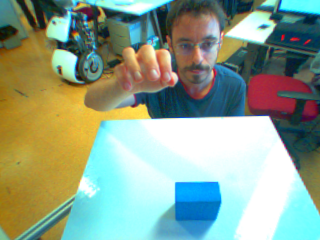
\includegraphics{grasp-00000169}
      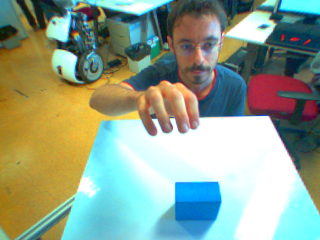
\includegraphics{grasp-00000170}
      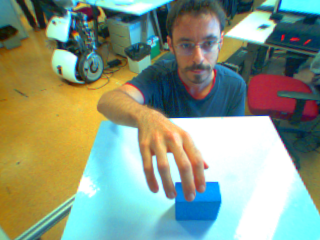
\includegraphics{grasp-00000171}
      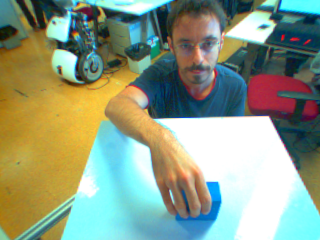
\includegraphics{grasp-00000173}
      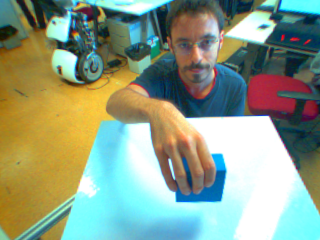
\includegraphics{grasp-00000177}
      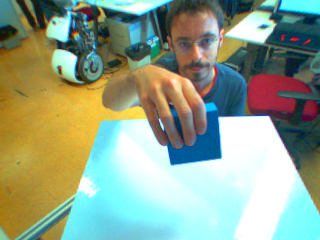
\includegraphics{grasp-00000180}
    } % end resizebox
    \label{fig:action_examples:grasp}
  } % end subfloat

  \subfloat[][Tap: the human moves the hand towards an object laterally and touches it, causing a motion effect.]{
    \resizebox{\linewidth}{!}{
      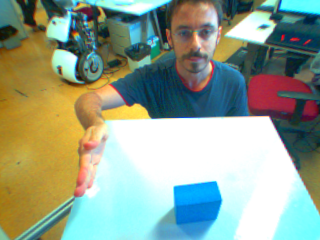
\includegraphics{tap-00000109}
      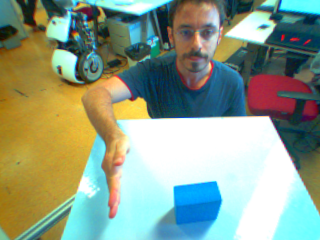
\includegraphics{tap-00000110}
      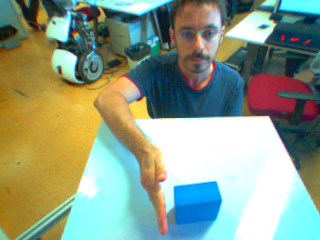
\includegraphics{tap-00000112}
      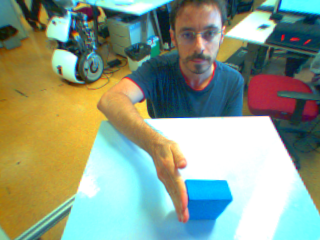
\includegraphics{tap-00000114}
      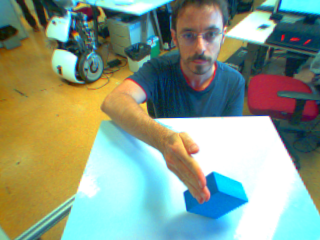
\includegraphics{tap-00000116}
      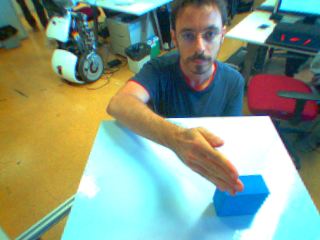
\includegraphics{tap-00000117}
    } % end resizebox
    \label{fig:action_examples:tap}
  } % end subfloat

  \subfloat[][Touch: the human moves the hand towards an object vertically, then touches it~(without grasping), then retracts the hand.]{
    \resizebox{\linewidth}{!}{
      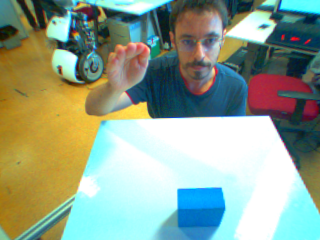
\includegraphics{touch-00000196}
      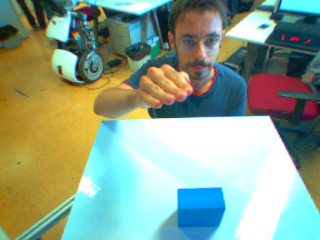
\includegraphics{touch-00000197}
      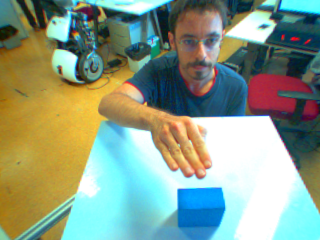
\includegraphics{touch-00000198}
      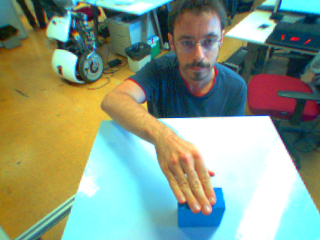
\includegraphics{touch-00000200}
      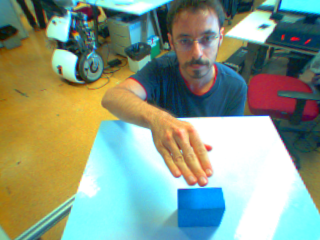
\includegraphics{touch-00000202}
      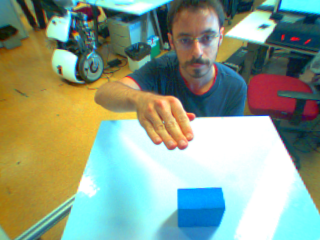
\includegraphics{touch-00000203}
    } % end resizebox
    \label{fig:action_examples:touch}
  } % end subfloat
  \caption{Examples of human actions from the point of view of the robot.}
  \label{fig:action_examples}
\end{figure*}

\section{Introduction}
\label{sec:intro}

% paragraph about HRC, understanding others, communication for cooperation
\IEEEPARstart{C}{ooperation}, or the ability of working successfully in groups, is a tenet of human society~\cite{turner:1975}.
This skill is acquired around the second year of life, when children develop an ability to coordinate themselves with peers or adult caregivers in shared problem-solving activities and social games.
This is achieved not only by mere behavioral coordination, but also by employing communicative strategies~\cite{melis:2010:rstb}.
In adulthood, sophisticated human team coordination and mutual understanding mechanisms take place~\cite{ramnani:2004:natureneuro}, making the most of the continuous observation of partners' actions, and also spoken language~(e.g., to transmit instructions or feedback).

% paragraph about social sobots, need for learning/adaptation of language
Even though social robots\footnote{A social robots is ``[a robot that is] able to communicate and interact with us, understand and even relate to us, in a personal way. [It] should be able to understand us and itself in social terms''~\cite{breazeal:2002:dsr}.} are becoming common in domestic and public environments, \hr{} teams still lag behind \hh{} teams in terms of effectiveness.
For robots, interpreting the actions of others and learning to describe them verbally~(for effective cooperation) is challenging.
The reason is that we cannot possibly model all the imaginable physical, verbal and non-verbal~(e.g., gestures) cues that can take place during \hri, due to the richness of language and the high variability of the real world outside of structured research laboratories and factories.
For this reason, it is necessary to have robots that \emph{learn} world elements and properties of language~\cite{iwahashi:2007:hri}, and the ability to link these verbal elements with other skills, such as other perceptual modalities~(e.g., vision of objects and other agents) and manipulation abilities~(e.g., grasping objects and placing them in order to achieve a goal)~\cite{steels:2003:trendscogsci}.

% paragraph introducing our approach + developmental robotics
Our work builds upon the intuition that a robot can use its previously-acquired knowledge of the world~(e.g., motor actions, objects properties, physical effects, verbal descriptions) to those situations where it observes a human agent performing familiar actions in a shared \hr{} scenario.
We follow the developmental robotics perspective~\cite{lungarella:2003:devrobsurvey,cangelosi:2015:devrobbook},
which takes inspiration from the progressive learning phenomena observed in children's mental development~(e.g., the understanding of language, the acquisition of manipulation skills, the understanding of others' actions), and investigates how to model the evolution and acquisition of these increasingly complex cognitive processes.

% paragraph summarizing our contributions and comparing with the GLU article
Extending on our recent work~\cite{saponaro:2017:glu}, we combine in this article robot ego-centric learning about language and object affordances~\cite{salvi:2012:smcb} with the observation of external agents by gesture recognition~\cite{saponaro:2013:crhri}.
Our novel contributions are:
(i)~a probabilistic method to fuse self-learned knowledge of language and object affordances, with socially aware information of others' physical actions~(in the form of uncertain soft evidence);
(ii)~experimental findings showing the reasoning power of our combined system, which is able to make inferences and predictions over affordances and words% by incorporating the estimation of external agents
; and
(iii)~the possibility of generating verbal descriptions from the estimated word probabilities and a pre-defined grammar, with emergence of non-trivial language properties such as congruent/incongruent conjunctions, synonyms between two consecutive sentences speaking about the same concepts.
Furthermore, we make our human action data and probabilistic reasoning code publicly available\footnote{\url{https://github.com/giampierosalvi/AffordancesAndSpeech}: the code from \cite{salvi:2012:smcb} has been extended to support the experiments in this study.}\footnote{\url{https://github.com/gsaponaro/tcds-gestures}: this page access will be made available at publication time.} in the interest of reproducibility.

This article is structured as follows.
In Sec.~\ref{sec:related_work} we briefly overview the literature on the interpretation and verbal description of others in different disciplines,
in Sec.~\ref{sec:method} we present our proposed method and its components,
in Sec.~\ref{sec:experimental_settings} we provide details and assumptions of the approach,
Sec.~\ref{sec:results} illustrates our results, and
in Sec.~\ref{sec:conclusions} we draw our concluding remarks.

%PHOTOS FROM OCTOBER 2017, NOT USED
% Below are the human-robot images from the external view (camera on a tripod)
% TODO: if we don't use them, purge seq2-*.png from the repo history
% \begin{figure*}
%     \centering
%     \subfloat
%     { 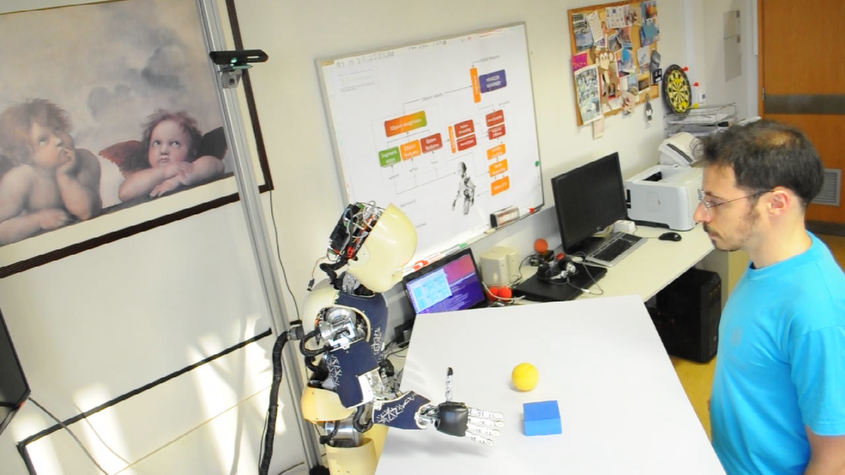
\includegraphics[width=\myWidth\linewidth]{seq2-grasp-11} } \quad
%     %
%     \subfloat
%     { 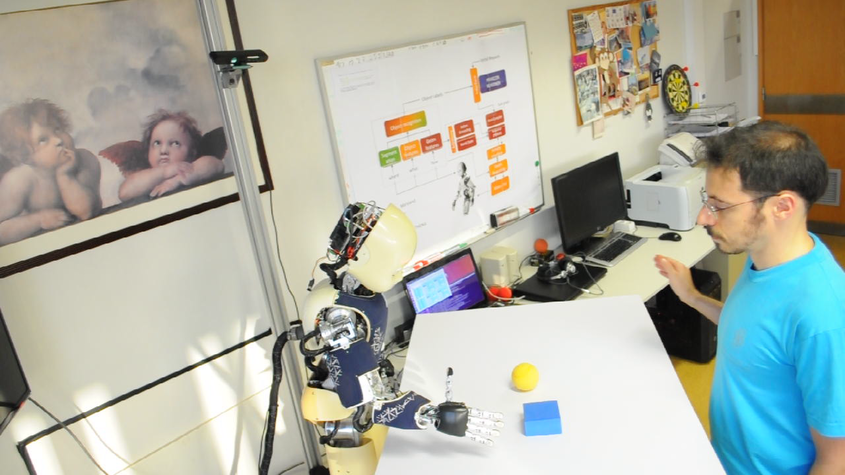
\includegraphics[width=\myWidth\linewidth]{seq2-grasp-12} } \quad
%     %
%     \subfloat
%     { 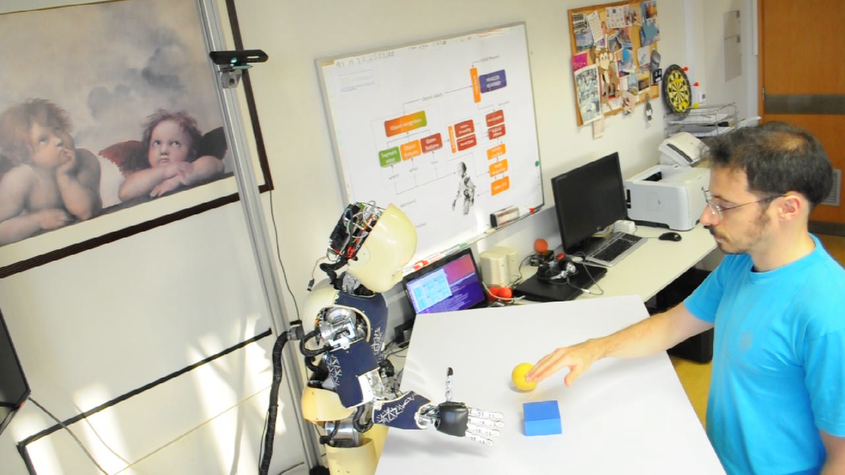
\includegraphics[width=\myWidth\linewidth]{seq2-grasp-13} } \\
%     %
%     \subfloat
%     { 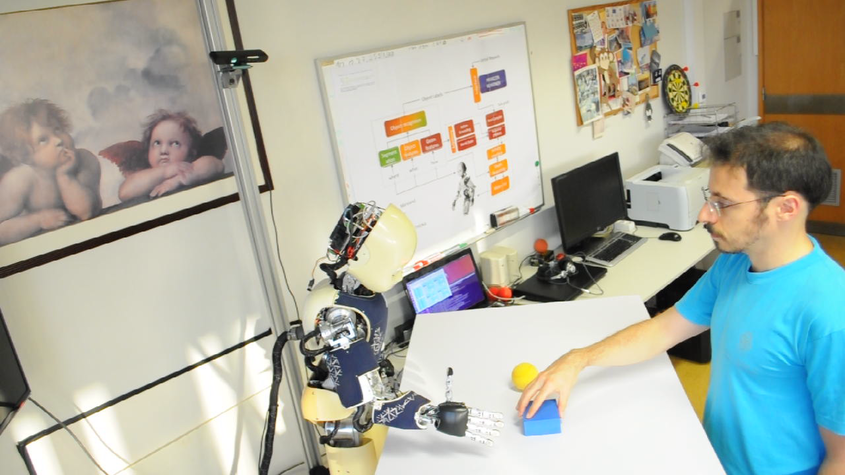
\includegraphics[width=\myWidth\linewidth]{seq2-grasp-14} } \quad
%     %
%     \subfloat
%     { 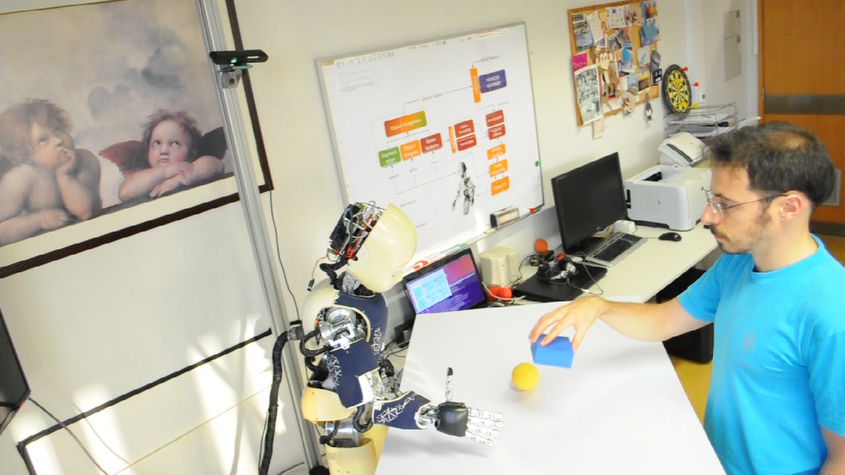
\includegraphics[width=\myWidth\linewidth]{seq2-grasp-15} } \quad
%     %
%     \subfloat
%     { 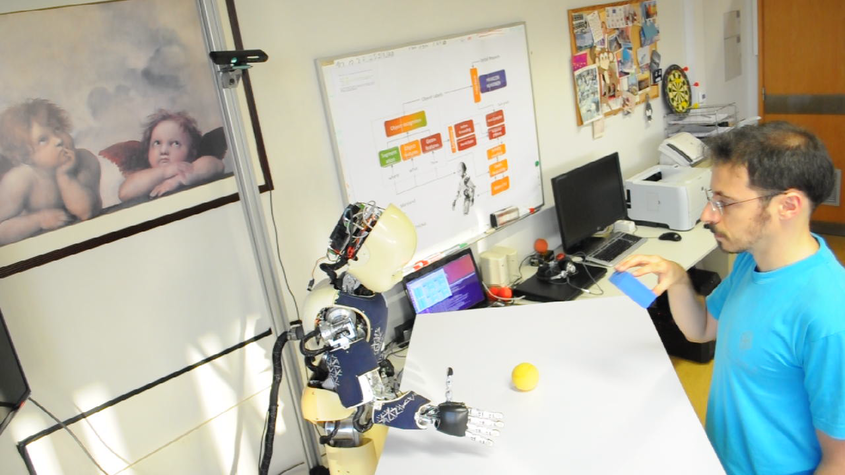
\includegraphics[width=\myWidth\linewidth]{seq2-grasp-16} }
%     \caption{grasp}
% \end{figure*}
%
% \begin{figure*}
%     \centering
%     \subfloat
%     { 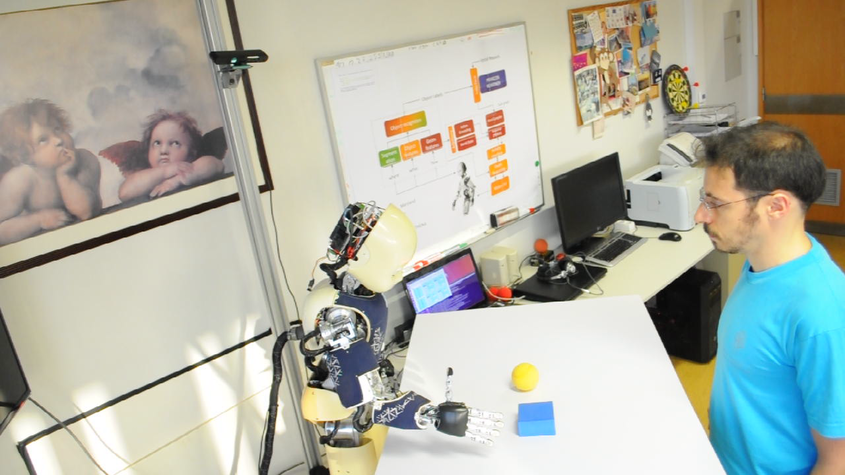
\includegraphics[width=\myWidth\linewidth]{seq2-tap-22} } \quad
%     %
%     \subfloat
%     { 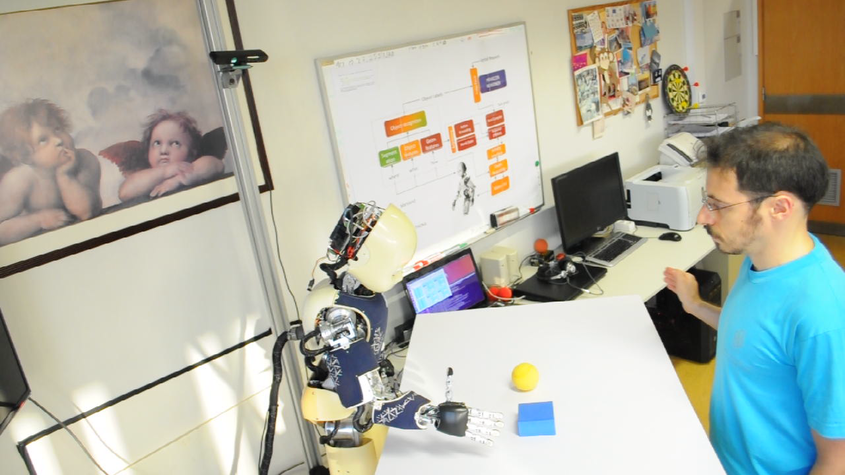
\includegraphics[width=\myWidth\linewidth]{seq2-tap-23} } \quad
%     %
%     \subfloat
%     { 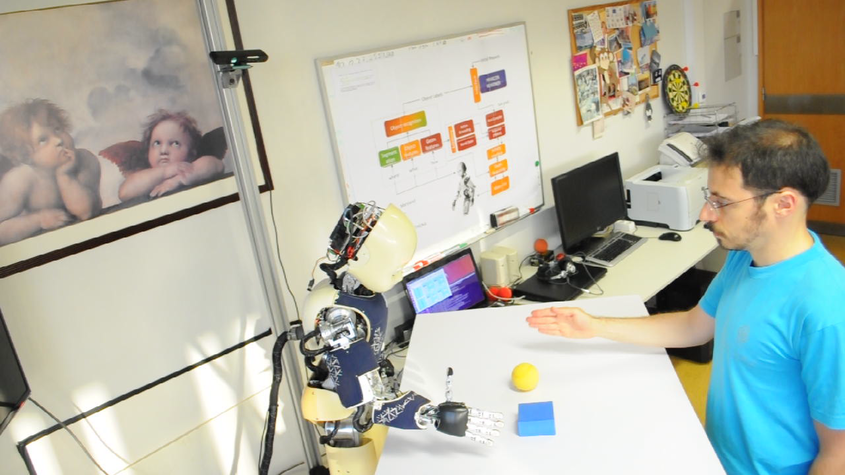
\includegraphics[width=\myWidth\linewidth]{seq2-tap-24} } \\
%     %
%     \subfloat
%     { 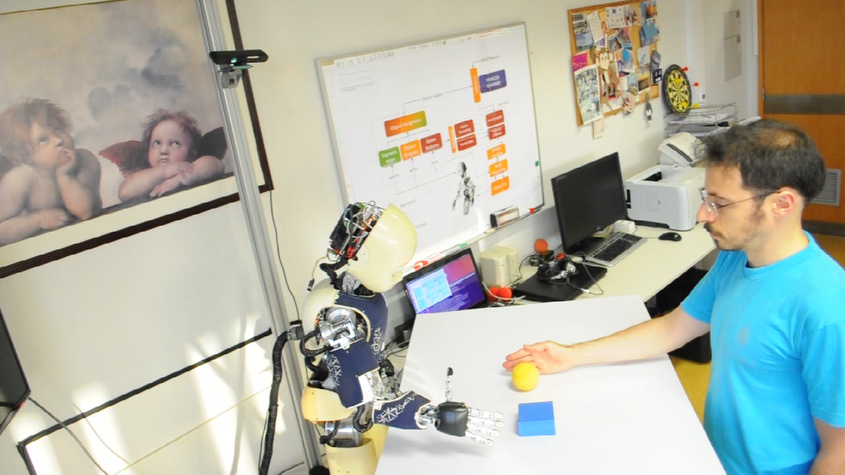
\includegraphics[width=\myWidth\linewidth]{seq2-tap-25} } \quad
%     %
%     \subfloat
%     { 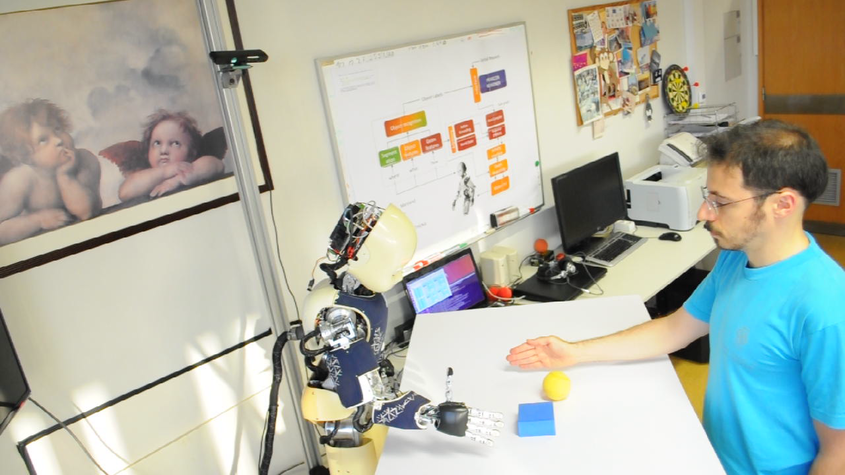
\includegraphics[width=\myWidth\linewidth]{seq2-tap-26} } \quad
%     %
%     \subfloat
%     { 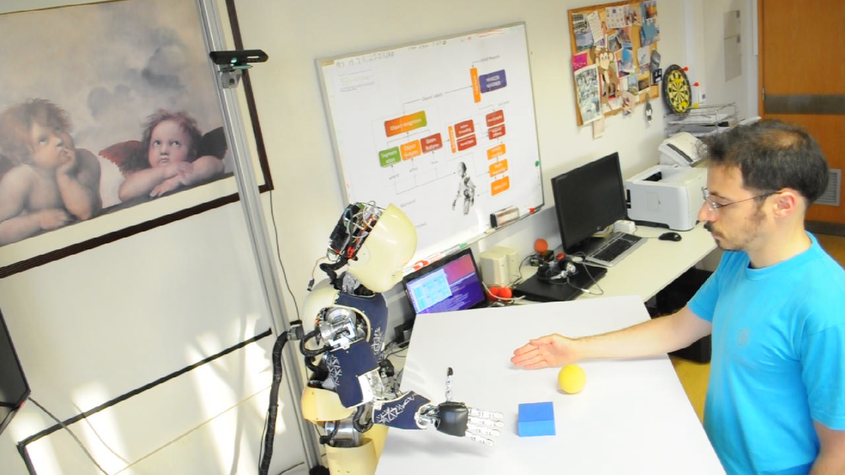
\includegraphics[width=\myWidth\linewidth]{seq2-tap-27} }
%     \caption{tap}
% \end{figure*}
%
% \begin{figure*}
%     \centering
%     \subfloat
%     { 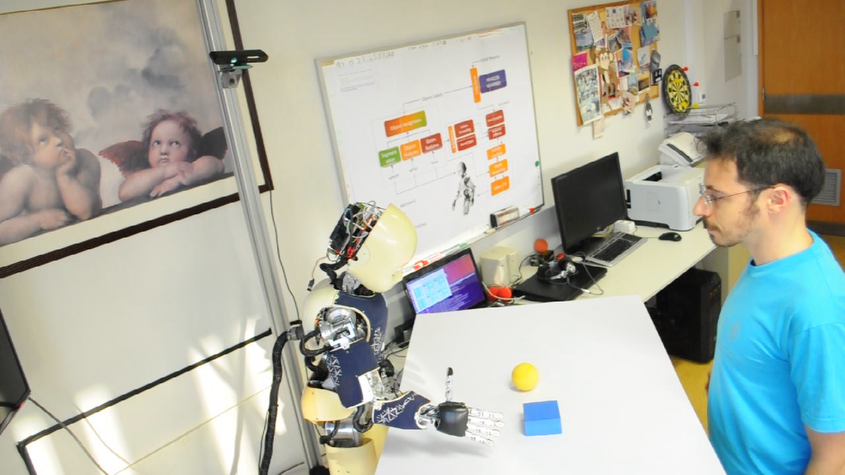
\includegraphics[width=\myWidthTwo\linewidth]{seq2-touch-2} } \quad
%     %
%     \subfloat
%     { 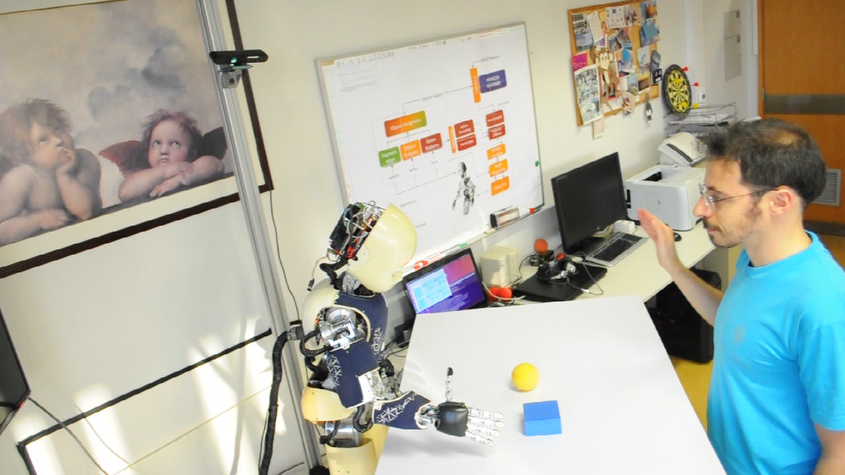
\includegraphics[width=\myWidthTwo\linewidth]{seq2-touch-3} } \quad
%     %
%     \subfloat
%     { 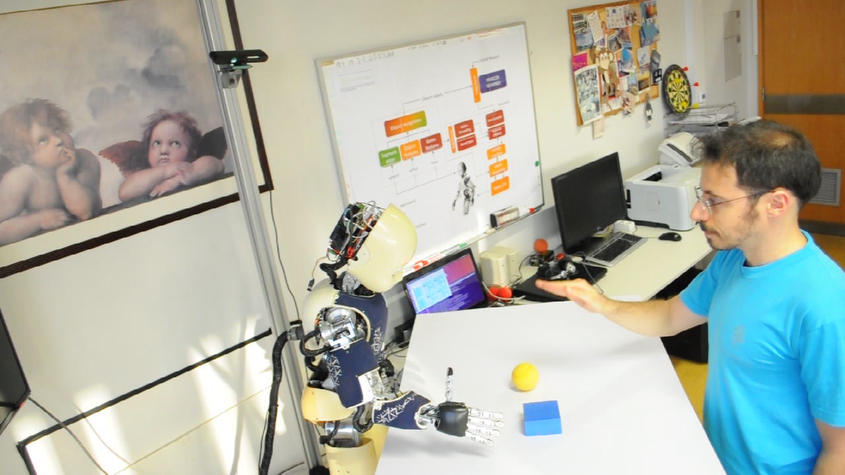
\includegraphics[width=\myWidthTwo\linewidth]{seq2-touch-4} } \quad
%     %
%     \subfloat
%     { 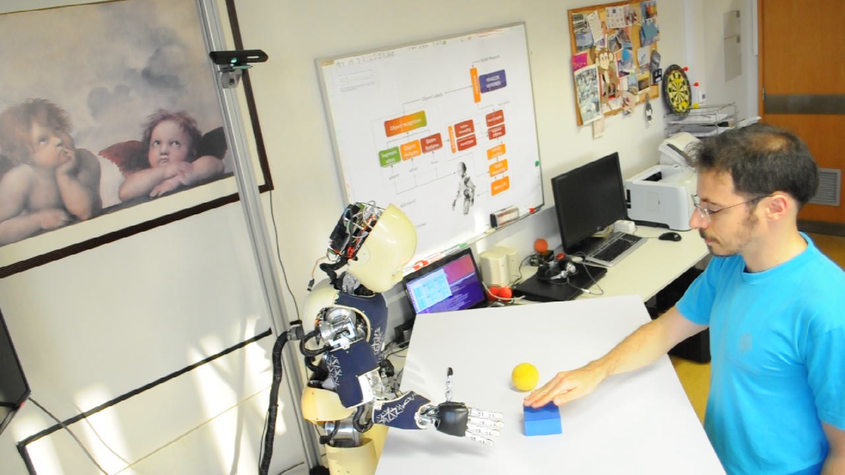
\includegraphics[width=\myWidthTwo\linewidth]{seq2-touch-5} } \\
%     %
%     \subfloat
%     { 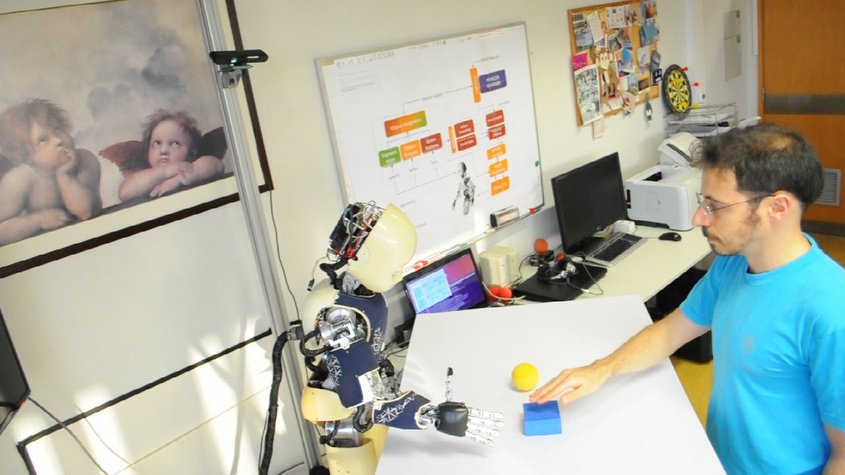
\includegraphics[width=\myWidthTwo\linewidth]{seq2-touch-6} } \quad
%     %
%     \subfloat
%     { 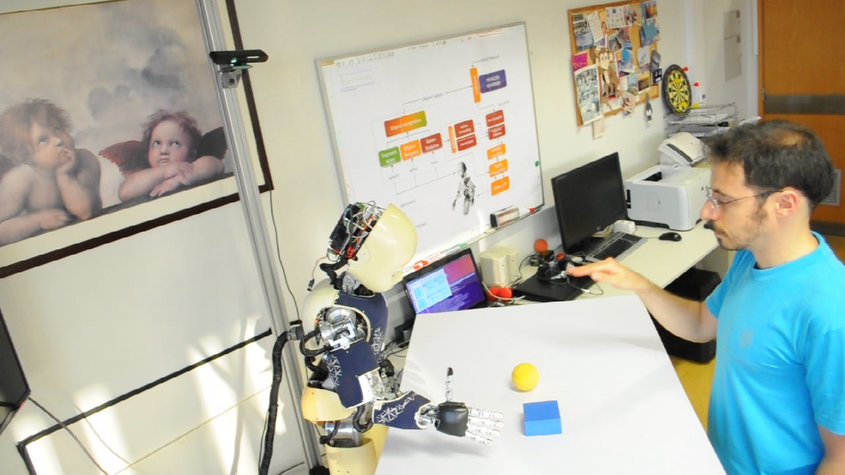
\includegraphics[width=\myWidthTwo\linewidth]{seq2-touch-7} } \quad
%     %
%     \subfloat
%     { 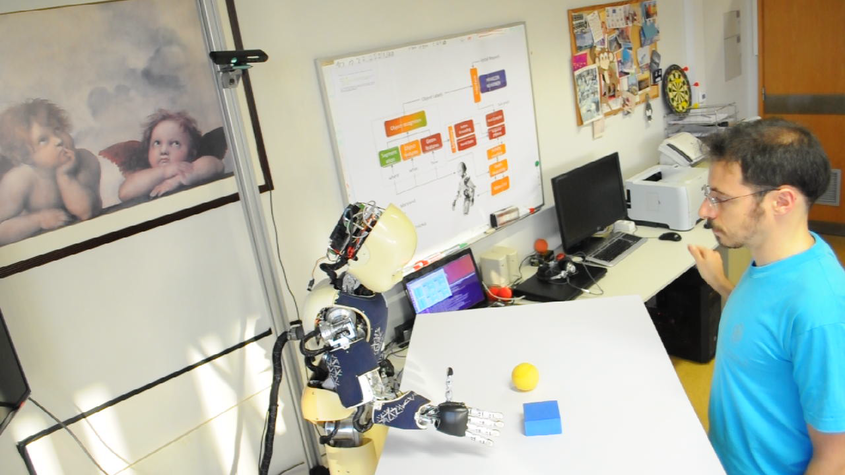
\includegraphics[width=\myWidthTwo\linewidth]{seq2-touch-8} } \quad
%     %
%     \subfloat
%     { 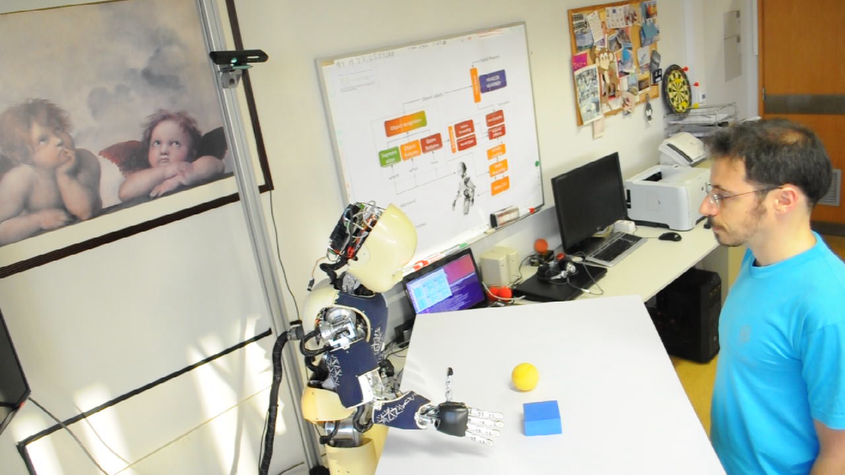
\includegraphics[width=\myWidthTwo\linewidth]{seq2-touch-9} }
%     \caption{touch}
% \end{figure*}
